
\documentclass[border=10pt, 12pt]{standalone}
\usepackage[svgnames]{xcolor}
\usepackage{amsmath}
\usepackage{pgfplots}
\pgfplotsset{compat=newest}
\usepackage[sfdefault]{FiraSans}
\usepackage{FiraMono}
\renewcommand*\familydefault{\sfdefault}
\begin{document}
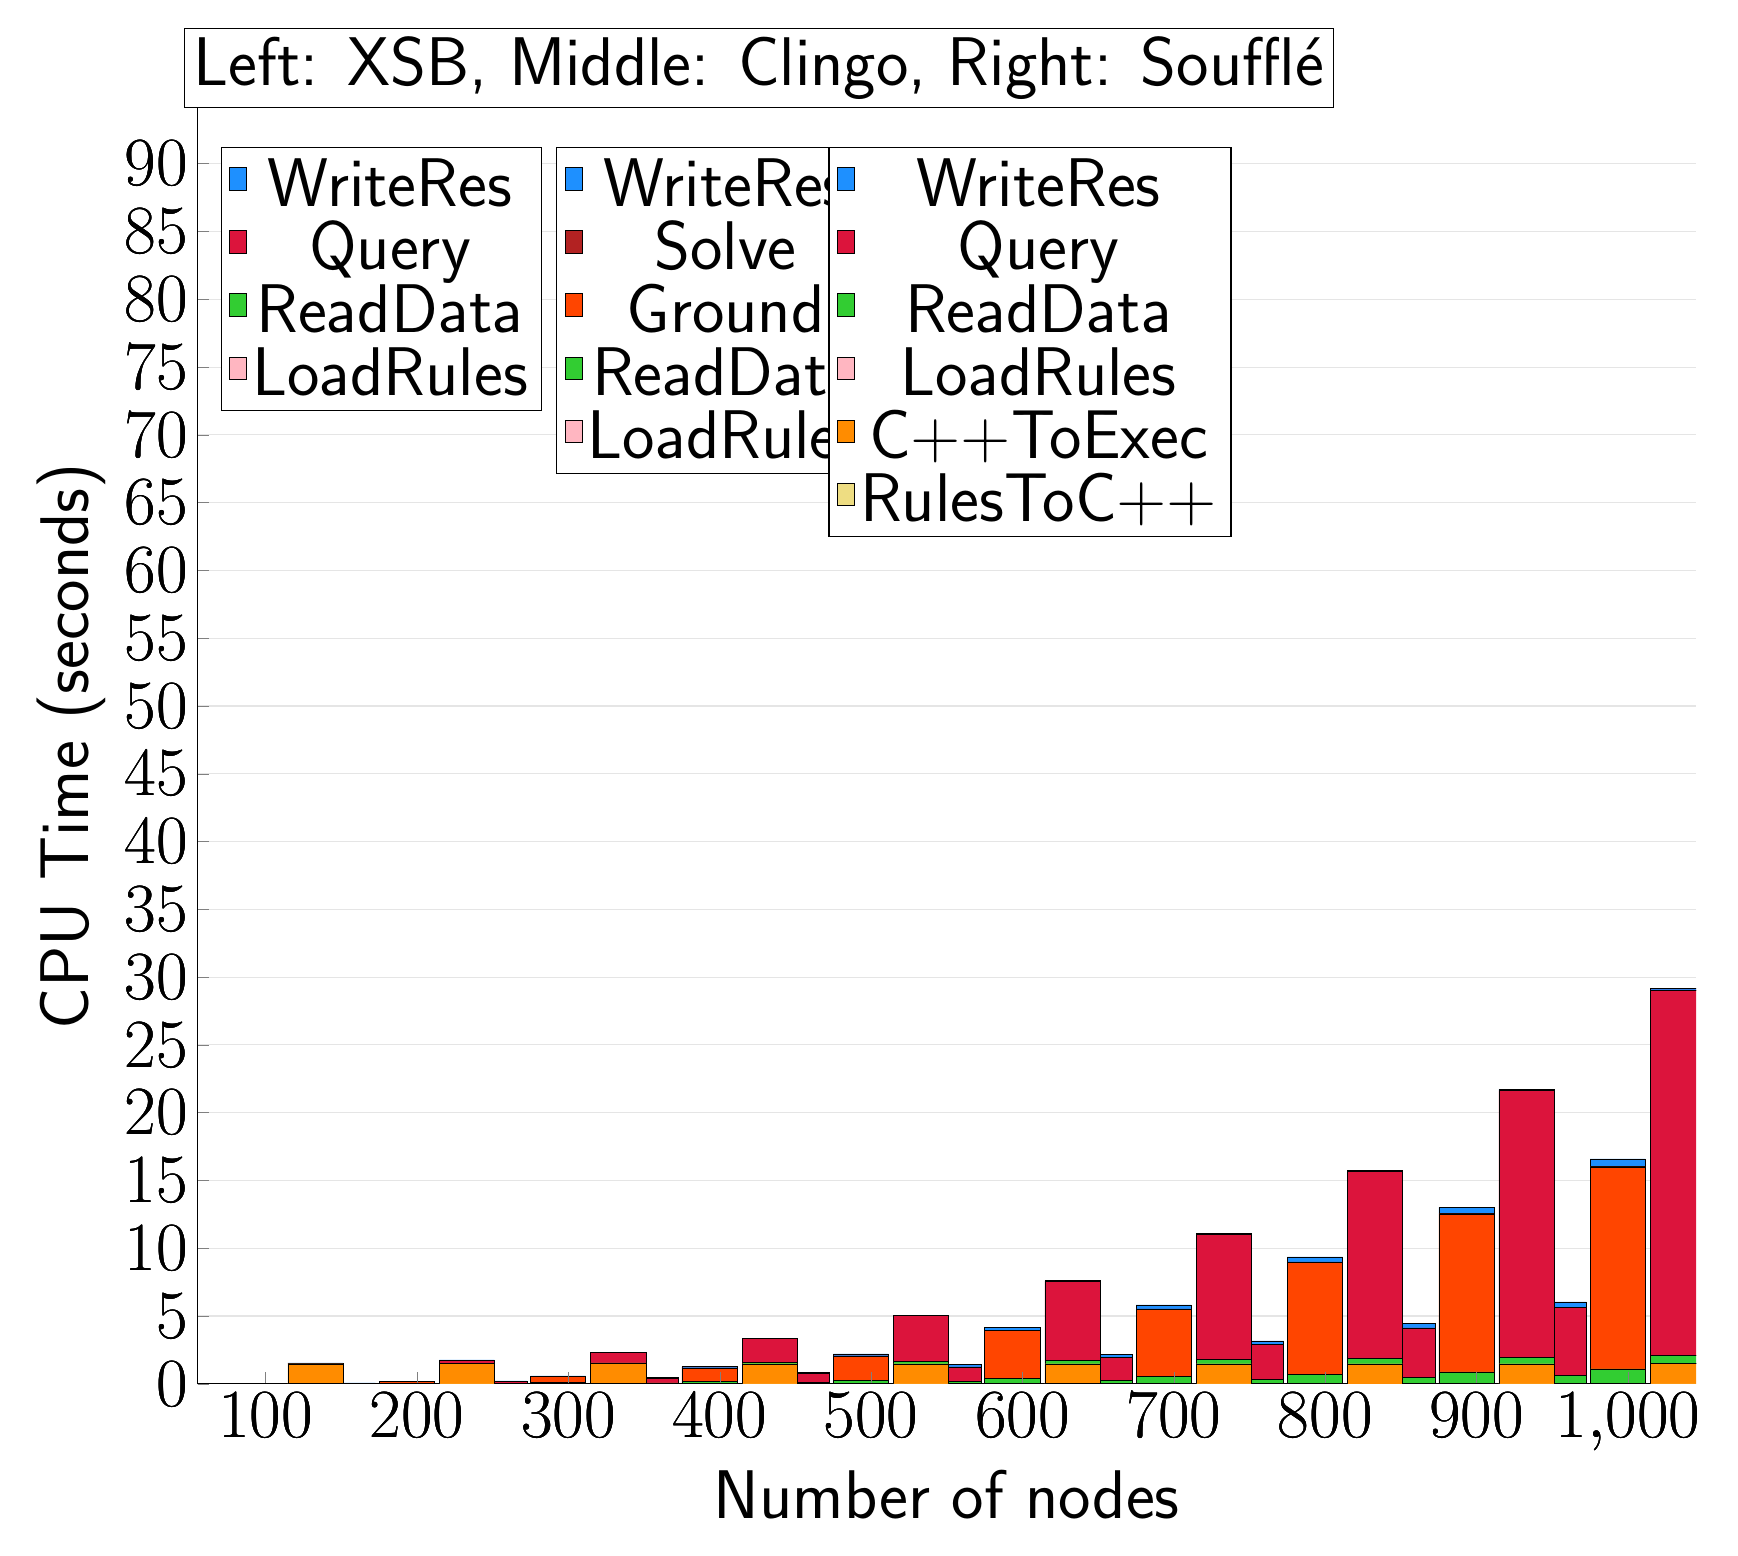
\begin{tikzpicture}
                        \begin{axis}[bar shift=-25pt, 
   ybar stacked,
   width=1.7\textwidth,
   bar width=0.7cm,
   ymajorgrids, tick align=inside,
   major grid style={draw=gray!20},
   xtick=data,
   ymin=0, ymax=94.08204,
   axis x line*=bottom,
   axis y line*=left,
   enlarge x limits=0.05,
   legend style={
       at={(0.23, 0.97)},
       anchor=north east,
       legend columns=1,
       font=\Huge,
   },
   ylabel={CPU Time (seconds)},
   xlabel={Number of nodes},
   label style={font=\Huge},
   tick label style={font=\Huge},
]
\addlegendimage{fill=DodgerBlue, draw=black, line width=0.2pt}
\addlegendentry{WriteRes}
\addlegendimage{fill=Crimson, draw=black, line width=0.2pt}
\addlegendentry{Query}
\addlegendimage{fill=LimeGreen, draw=black, line width=0.2pt}
\addlegendentry{ReadData}
\addlegendimage{fill=LightPink, draw=black, line width=0.2pt}
\addlegendentry{LoadRules}
\addplot +[fill=LightPink, draw=black, line width=0.2pt] coordinates {
(100, 0.000547)
(200, 0.0005527999999999998)
(300, 0.0005453999999999996)
(400, 0.0005456000000000009)
(500, 0.0005463999999999998)
(600, 0.000547799999999999)
(700, 0.0005491999999999996)
(800, 0.0005476000000000002)
(900, 0.0005388000000000001)
(1000, 0.0005492000000000002)
};
\addplot +[fill=LimeGreen, draw=black, line width=0.2pt] coordinates {
(100, 0.0040349999999999995)
(200, 0.0169408)
(300, 0.039872399999999995)
(400, 0.0743898)
(500, 0.12167779999999999)
(600, 0.1819734)
(700, 0.2590598)
(800, 0.3531926)
(900, 0.4652198)
(1000, 0.6027292)
};
\addplot +[fill=Crimson, draw=black, line width=0.2pt] coordinates {
(100, 0.0053082)
(200, 0.0414406)
(300, 0.13832039999999998)
(400, 0.3222674)
(500, 0.6293390000000001)
(600, 1.0751302)
(700, 1.7041456)
(800, 2.5593396)
(900, 3.655734)
(1000, 5.021369)
};
\addplot +[fill=DodgerBlue, draw=black, line width=0.2pt] coordinates {
(100, 0.00412)
(200, 0.017191799999999997)
(300, 0.036710999999999994)
(400, 0.06583419999999998)
(500, 0.10668700000000002)
(600, 0.15758059999999996)
(700, 0.19956759999999996)
(800, 0.25718620000000014)
(900, 0.32747080000000006)
(1000, 0.4123279999999999)
};
\end{axis}

\begin{axis}[bar shift=-3.7pt, 
   ybar stacked,
   width=1.7\textwidth,
   bar width=0.7cm,
   ymajorgrids, tick align=inside,
   major grid style={draw=none},
   xtick=data,
   ymin=0, ymax=94.08204,
   axis x line*=none,
   axis y line*=none,
   enlarge x limits=0.05,
   legend style={
       at={(0.454, 0.97)},
       anchor=north east,
       legend columns=1,
       font=\Huge,
   },
   label style={font=\Huge},
   tick label style={font=\Huge},
]
\addlegendimage{fill=DodgerBlue, draw=black, line width=0.2pt}
\addlegendentry{WriteRes}
\addlegendimage{fill=FireBrick, draw=black, line width=0.2pt}
\addlegendentry{Solve}
\addlegendimage{fill=OrangeRed, draw=black, line width=0.2pt}
\addlegendentry{Ground}
\addlegendimage{fill=LimeGreen, draw=black, line width=0.2pt}
\addlegendentry{ReadData}
\addlegendimage{fill=LightPink, draw=black, line width=0.2pt}
\addlegendentry{LoadRules}
\addplot +[fill=LightPink, draw=black, line width=0.2pt] coordinates {
(100, 0.0)
(200, 0.0)
(300, 0.0)
(400, 0.0)
(500, 0.0)
(600, 0.0)
(700, 0.0)
(800, 0.0)
(900, 0.0)
(1000, 0.0)
};
\addplot +[fill=LimeGreen, draw=black, line width=0.2pt] coordinates {
(100, 0.010000000000000009)
(200, 0.040000000000000036)
(300, 0.09200000000000003)
(400, 0.16999999999999998)
(500, 0.266)
(600, 0.38)
(700, 0.544)
(800, 0.6920000000000001)
(900, 0.8780000000000001)
(1000, 1.096)
};
\addplot +[fill=OrangeRed, draw=black, line width=0.2pt] coordinates {
(100, 0.018000000000000016)
(200, 0.12999999999999995)
(300, 0.442)
(400, 1.002)
(500, 1.7899999999999998)
(600, 3.5660000000000003)
(700, 4.974)
(800, 8.280000000000001)
(900, 11.652000000000003)
(1000, 14.904000000000002)
};
\addplot +[fill=FireBrick, draw=black, line width=0.2pt] coordinates {
(100, 0.0020000000000000018)
(200, 0.0)
(300, 0.006000000000000005)
(400, 0.008000000000000007)
(500, 0.0060000000000000496)
(600, 0.009999999999999787)
(700, 0.016000000000000014)
(800, 0.02199999999999993)
(900, 0.023999999999999844)
(1000, 0.03999999999999923)
};
\addplot +[fill=DodgerBlue, draw=black, line width=0.2pt] coordinates {
(100, -0.0020000000000000018)
(200, 0.02200000000000002)
(300, 0.04599999999999993)
(400, 0.09400000000000008)
(500, 0.14600000000000007)
(600, 0.21000000000000013)
(700, 0.28799999999999987)
(800, 0.36399999999999977)
(900, 0.47000000000000003)
(1000, 0.554000000000002)
};
\end{axis}

\begin{axis}[bar shift=18pt, 
   ybar stacked,
   width=1.7\textwidth,
   bar width=0.7cm,
   ymajorgrids, tick align=inside,
   major grid style={draw=none},
   xtick=data,
   ymin=0, ymax=94.08204,
   axis x line*=none,
   axis y line*=none,
   enlarge x limits=0.05,
   legend style={
       at={(0.69, 0.97)},
       anchor=north east,
       legend columns=1,
       font=\Huge,
   },
   label style={font=\Huge},
   tick label style={font=\Huge},
]
\addlegendimage{fill=DodgerBlue, draw=black, line width=0.2pt}
\addlegendentry{WriteRes}
\addlegendimage{fill=Crimson, draw=black, line width=0.2pt}
\addlegendentry{Query}
\addlegendimage{fill=LimeGreen, draw=black, line width=0.2pt}
\addlegendentry{ReadData}
\addlegendimage{fill=LightPink, draw=black, line width=0.2pt}
\addlegendentry{LoadRules}
\addlegendimage{fill=DarkOrange, draw=black, line width=0.2pt}
\addlegendentry{C++ToExec}
\addlegendimage{fill=LightGoldenrod, draw=black, line width=0.2pt}
\addlegendentry{RulesToC++}
\addplot +[fill=LightGoldenrod, draw=black, line width=0.2pt] coordinates {
(100, 0.006000000000000001)
(200, 0.0020000000000000005)
(300, 0.006000000000000001)
(400, 0.0020000000000000005)
(500, 0.0020000000000000005)
(600, 0.006000000000000001)
(700, 0.0020000000000000005)
(800, 0.0)
(900, 0.0020000000000000005)
(1000, 0.0020000000000000005)
};
\addplot +[fill=DarkOrange, draw=black, line width=0.2pt] coordinates {
(100, 1.472)
(200, 1.48)
(300, 1.4739999999999998)
(400, 1.474)
(500, 1.466)
(600, 1.47)
(700, 1.47)
(800, 1.476)
(900, 1.476)
(1000, 1.478)
};
\addplot +[fill=LightPink, draw=black, line width=0.2pt] coordinates {
(100, 0.000163)
(200, 0.0002028)
(300, 0.0001538)
(400, 0.0001672)
(500, 0.0001664)
(600, 0.00018559999999999998)
(700, 0.0001746)
(800, 0.00011920000000000001)
(900, 0.0001364)
(1000, 0.0001806)
};
\addplot +[fill=LimeGreen, draw=black, line width=0.2pt] coordinates {
(100, 0.014233)
(200, 0.0424916)
(300, 0.06924559999999999)
(400, 0.1118292)
(500, 0.1647)
(600, 0.2280462)
(700, 0.3022158)
(800, 0.380132)
(900, 0.47982440000000004)
(1000, 0.5931984)
};
\addplot +[fill=Crimson, draw=black, line width=0.2pt] coordinates {
(100, 0.0428654)
(200, 0.2289376)
(300, 0.7474725999999999)
(400, 1.7568139999999999)
(500, 3.4065500000000006)
(600, 5.860647999999999)
(700, 9.2762)
(800, 13.80716)
(900, 19.6714)
(1000, 26.983659999999997)
};
\addplot +[fill=DodgerBlue, draw=black, line width=0.2pt] coordinates {
(100, 0.0014314)
(200, 0.004534999999999999)
(300, 0.009944999999999999)
(400, 0.017435799999999998)
(500, 0.0270044)
(600, 0.038553000000000004)
(700, 0.052592799999999995)
(800, 0.0686184)
(900, 0.086324)
(1000, 0.1069372)
};
\end{axis}


\node[anchor=south, draw, fill=white] at (rel axis cs:0.42,1) {\Huge Left: XSB, Middle: Clingo, Right: Soufflé};
\end{tikzpicture}
\end{document}
                    